%
% TTÜ Style Thesis template for LaTeX
%
% Public Version 1.1
% 2019 Adjusted by Frank Korving for his TTÜ Bachelor Thesis, with contributions from Sander Arnus
%
% Public version 1.0
% 2010 - 2013 Thijs Nugteren and Joos Buijs for TU/e Master Thesis
%
% THIS IS THE MAIN FILE (i.e. compile this file, compiling the others directly won't work)
%
\documentclass[12pt, a4paper]{report}

% all the other includes etc. are done in the thesis.sty file.
\hbadness=10000
\hfuzz=50pt
\usepackage{thesis}

%
% These commands need to be defined in order to produce a correct and personalized document
%
\newcommand{\doctitle}{ Thesis/project title}
\newcommand{\docsubtitle}{MASTERS OF SCIENCE IN COMPUTER SCIENCE AND ENGINEERING}

\newcommand{\me}{Author name}
\newcommand{\studentcode}{Student ID}
\newcommand{\university}{CHITTAGONG UNIVERSITY OF ENGINEERING AND TECHNOLOGY}
\newcommand{\school}{School of ...}
\newcommand{\department}{\textcolor{astral}{Department of computer Science and Engineering(CSE)}}

\newcommand{\supervisor}{Name of superviosor}
\newcommand{\supervisortitle}{PhD}
\newcommand{\cosupervisor}{b}
\newcommand{\cosupervisortitle}{MSC}
\newcommand{\keywords}{Important, comma, separated, keywords, applicable, to, your, thesis}
\newcommand{\version}{0.1 version}
\newcommand{\monthYear}{Month Year}
\newcommand{\Year}{Year}
\newcommand{\signatureDate}{13, 01, 2020}

\author{\me}

%
% PDF settings
%
\hypersetup
{
    pdfauthor={\me},
    pdfsubject={\doctitle},
    pdfkeywords={\keywords}
}

\begin{document}
\renewcommand\baselinestretch{1.2}
\baselineskip=18pt plus1pt
\pagenumbering{roman}
\begin{titlepage}
\vspace*{\fill}
\begin{center}

\textbf{\LARGE Thesis Title}
\\[ 0.5 in]
by\\ [0.1in] \textcolor{astral}{Author's Name\\ [0.05in] Roll No: Student ID}
\\[1 in]
\end{center}
\begin{center}
   A thesis submitted for the partial fulfillment of the requirement for the degree of 

\textit{MASTER OF SCIENCE IN COMPUTER SCIENCE AND ENGINEERING} 
\end{center}
\begin{figure}[ht]
\centering

\includegraphics[width=2 in]{figures/logo.jpg}
\centering
\end{figure} 
\begin{center}
\large{Department of Computer Science and Engineering(CSE)}
\\[0.05in]
CHITTAGONG UNIVERSITY OF ENGINEERING AND TECHNOLOGY
\\[0.05in]
Chattogram-4349, Bangladesh
\\[0.05in]
January, 2020
\end{center}
\vspace*{\fill}

\end{titlepage}

%\include {firstpage}
\normalsize
%%%%%%%%%%%%%%%%%%%%%%%
% Certification page holding signature of the board member
\begin{center}
    \textbf{\LARGE{CERTIFICATION}}
\end{center}
%\newline\newline\newline\newline\newline
The thesis titled  \textbf{"Thesis Title"} submitted by \textbf{Author's Name}, Roll No \textbf{Student ID}, Session \textbf{(Author's session) 2014-2015}
%%%% Put your own session
has been accepted as satisfactory in partial fulfillment of the requirement for the degree of  MASTER OF SCIENCE IN COMPUTER SCIENCE \& ENGINEERING  on   -/-/-
% Please add the following required packages to your document preamble:
% \usepackage[normalem]{ulem}
% \useunder{\uline}{\ul}{}
\begin{table}[H]
\centering
\label{tab:my-table}
\begin{tabular}{ll}
\multicolumn{2}{c}{\textbf{BOARD OF EXAMINER}}                                                                                                                                                                                                                                        \\
                                                                                                                                                                                                                    &                                                                 \\
1. \_\_\_\_\_\_\_\_\_\_\_\_\_\_\_\_\_\_\_\_\_\_\_\_\_\_\_\_\_\_\_\_\_\_\_\_\_\_\_\_\_\_\_\_\_\_\_\_                                                                                                                 &                                                                 \\
\begin{tabular}[c]{@{}l@{}}Dr. M X Y Z\\ Professor\\ Department of Computer Science \& Engineering\\ Chittagong University of Engineering \& Technology\\ Chattogram- 4349, Bangladesh.\end{tabular} & \begin{tabular}[c]{@{}l@{}}Chairman\\ (Supervisor)\end{tabular} \\
                                                                                                                                                                                                                    &                                                                 \\
                                                                                                                                                                                                                    4. \_\_\_\_\_\_\_\_\_\_\_\_\_\_\_\_\_\_\_\_\_\_\_\_\_\_\_\_\_\_\_\_\_\_\_\_\_\_\_\_\_\_\_\_\_\_\_\_                                                                                                                 &                                                                 \\
\begin{tabular}[c]{@{}l@{}}Dr. SST\\ Professor \& Head\\ Department of Computer Science \& Engineering\\ Chittagong University of Engineering \& Technology\\ Chattogram- 4349, Bangladesh.\end{tabular}    & \begin{tabular}[c]{@{}l@{}}Member\\ (Ex-Officio)\end{tabular}   \\
                                                                                                                                                                                                                    &                                                                 \\
3. \_\_\_\_\_\_\_\_\_\_\_\_\_\_\_\_\_\_\_\_\_\_\_\_\_\_\_\_\_\_\_\_\_\_\_\_\_\_\_\_\_\_\_\_\_\_\_\_                                                                                                                 &                                                                 \\
\begin{tabular}[c]{@{}l@{}}Dr. PQR\\ Professor\\ Department of Computer Science \& Engineering\\ Chittagong University of Engineering \& Technology\\ Chattogram- 4349, Bangladesh.\end{tabular}  & Member                                                          \\
                                                                                                                                                                                                                    &                                                                 \\
4. \_\_\_\_\_\_\_\_\_\_\_\_\_\_\_\_\_\_\_\_\_\_\_\_\_\_\_\_\_\_\_\_\_\_\_\_\_\_\_\_\_\_\_\_\_\_\_\_                                                                                                                 &                                                                 \\
\begin{tabular}[c]{@{}l@{}}Dr. GHK\\ Professor\\ Department of Computer Science \& Engineering\\ Chittagong University of Engineering \& Technology\\ Chattogram- 4349, Bangladesh.\end{tabular}            & Member                                                          \\
                                                                                                                                                                                                                    &                                                                 \\

5. \_\_\_\_\_\_\_\_\_\_\_\_\_\_\_\_\_\_\_\_\_\_\_\_\_\_\_\_\_\_\_\_\_\_\_\_\_\_\_\_\_\_\_\_\_\_\_\_                                                                                                                 &                                                                 \\
\begin{tabular}[c]{@{}l@{}}Dr. MNO\\ Professor\\ Department of Computer Science and Engineering\\ XTR University of Engineering \& Technology\\ XTR- 6205, Bangladesh\end{tabular}               & \begin{tabular}[c]{@{}l@{}}Member\\ (External)\end{tabular}    
\end{tabular}
\end{table}
\pagebreak
%%%%%%%%%%%%%%
% include author's declaration page with signature
\chapter*{\centerline{Author's Declaration of Originality}}\label{chapter:declaration}
\hfill \\
I hereby certify that I am the sole author of this thesis. All the used materials, references
to the literature and the work of others have been referred to. This thesis or any part of it has not been
submitted elsewhere for the award of any degree or diploma.

\vskip1in
\begin{flushleft}
\begin{tabular}{p{2.0cm}p{6.0cm}p{4.0cm}}
  Author: & \me & ......................................\\
  && \hfill(signature)\\
  Date: & \signatureDate &\\
  \\
  \\

% Uncomment the following to add supervisor declaration
%  \multicolumn{3}{l}{The thesis adheres to all specified requirements}\\
%  \hfill \\
%  Supervisor: & \supervisor & ......................................\\
%  && \hfill(signature)\\
%  Date: & \signatureDate &\\


\end{tabular}
\end{flushleft}
\pagebreak
%%%%%%%%%%%%%%%%%%%%%%%%%%%%%%%%%%%%
% include dedication page
\label{chapter:Dedication}
\begin{center}
  
    \vspace*{\fill}
  \itshape {\large{It is my genuine gratefulness and warmest regard that \\I dedicate this work to my beloved} \\
 
 \Large{ \bfseries{Father and Mother}}}
    \vspace*{\fill}
\end{center}
\clearpage

\pagebreak
\phantomsection

\setcounter{tocdepth}{3}    % Sets maximum depth of Table Of Contents
%%%%%%%%%%%%%%%%%%%%%%%%%%%%%%%%%%%%%%%%%%%%%%
%Table of contents, list of table, list of figures, list of algorithms, list of terms and abbreviation
\renewcommand{\contentsname}{Table of Contents}
\tableofcontents
\clearpage \phantomsection
\setcounter{figure}{0}
\addcontentsline{toc}{chapter}{List of Figures}
\listoffigures

\clearpage \phantomsection
\addcontentsline{toc}{chapter}{List of Tables}
\listoftables
\clearpage \phantomsection

\addcontentsline{toc}{chapter}{List of Algorithms}
\begin{spacing}{0.25}\listofalgorithms\end{spacing}
\setlength\parskip{\bigskipamount}
\chapter*{{List of Terms and Abbreviations}}\label{chapter:terms}
\begin{longtable}{p{3cm}p{10cm}}
VFA& Visual Focus of Attention\\
FDM&Face Detection Module\\
GDTM&Gaze Detection and Tracking Module\\
GAwM&Gaze Awareness Module\\
RRCM&Robot Control and Response Module\\
H& Human\\
R& Robot\\
\end{longtable}
\addtocounter{table}{-1} 
\addcontentsline{toc}{chapter}{Terms and Abbreviation}

\chapter*{\centerline{Acknowledgement}}\label{chapter:acknowledge}
\addcontentsline{toc}{chapter}{Acknowledgement}
I am overwhelmed to get this opportunity to express my gratitude to those whose constant support and encouragement lead me to the completion of my thesis on human robot interaction.
First and foremost, I feel immense proud to express my heartfelt respect and deepest sense of gratitude to my supervisor, Prof. Dr. Mohammed Moshiul Hoque for his scholarly guidance, instruction, constructive criticism, valuable suggestions, supervision, inspiration, untiring assistance in all phases of the research work and in the preparation of the report manuscript. Without his pedagogic supervision, heartfelt help, unfailing attention, and constructive criticism this report would not have seen the light of the day. I am ever grateful to the honorable examination board member for their valuable suggestion, helpful comment, and affectionate feeling.

I am incredibly grateful to all the faculty members
and the staff of department of CSE, CUET for their support. My friends, colleagues and several students  of CUET deserves special thanks for their assistance to make this work possible.
I express my cordial respect and sincere appreciation to my parents for their unforgettable kind co-operation, constructive suggestions, sacrifice, and cordial support in all spheres of the working period.

 Finally, all praises to Allah, the Almighty because it is He, who give me the strength and courage to accomplish the task and achieve the goal. 

\chapter*{\centerline{Abstract}}\label{chapter:abstract}
\addcontentsline{toc}{chapter}{Abstract}
\vspace{-2.5em}
The thesis is in ... and contains ... pages of text, ... chapters, ... figures, ... tables.
The abstract view of the thesis, objective and final result should be emphasized. PLEASE FOLLOW YOUR Supervisor's suggestions.

\textbf{Keywords:} Keywords of the thesis. 
\pagebreak

\chapter{Introduction}\label{chapter:chapter1}
\onehalfspacing
\setcounter{page}{0}
\pagenumbering{arabic}   %from here on, start the 'real' page numbering, from 1, with normal digits
Some basic ways to manipulate text are \textit{italics}, \textbf{bold}, and \textcolor{blue}{colored text}. One can reference Figures (see Figure \ref{logo} for an example) as well as cite references which are defined in the \textit{references.bib} file.\cite{spectre,example-reference} 
\begin{center}
    \begin{figure}[ht] \label{logo}
\centering

\includegraphics[width=2 in]{figures/logo.jpg}
\centering
\end{figure} 
\end{center}
The \textit{Bibliography}, \textit{List of Figures} and \textit{List of Tables} are all automatically generated and references will be updated automatically as well. This means that if you've defined a citation but are not referencing it, it will not appear in the \textit{Bibliography}. This also means that any Figure / Table / Citations numbers are automatically updated as well. Numbering is done by order-of-appearance.
\section{Item, enumerate, and list}
One can create an itemized list:
(i) \begin{itemize}
    \item item a
    \item item b
    \item ...
\end{itemize}
(ii)
\begin{itemize}[label=\ding{212}]
\item First
\item Second
\end{itemize}
Or enumerate them:
(i) \begin{enumerate}
    \item item x
    \item item y
    \item ...
\end{enumerate}


(ii) \begin{enumerate}[label=\roman*]
  \item item x
  \item item y
  \item item ..
\end{enumerate}

(iii) \begin{enumerate}[label=\Roman*]
\item item x
  \item item y
  \item item ..
\end{enumerate}
or listed them

\begin{list}{$\circ$}{}  
\item A  
\item B  
\end{list}
Another example are showing below:
\begin{itemize}

\item[$\checkmark$] This will give a checkmark bullet.

\item[$\square$] This will give a hollow square bullet.

\item[$\blacksquare$] This will give a filled square bullet.

\item[$\bigstar$] This will give you a bigstar bullet.

\end{itemize}
We can use variables set in the \textit{main.tex} file to render values like our title (\doctitle) or supervisor names (\textbf{Supervisor}: \supervisor, \textbf{Co-supervisor}: \cosupervisor{}).

You may add following sections in this chapter.
\begin{itemize}
    \item objective
    \item motivation
    \item challenges
    \item Design approach
    \item contribution
    \item Organize of the thesis
    \item Summary
\end{itemize}
\section{Section, sub section, sub sub section, section without listing in the TOC}
\section{Section} \label{sec}
subsection will be under section.
\subsection{Sub section}\label{sub}
After subsection you can add "subsubsection"
\section{section/subsection without listing in TOC}
to do so you need to add "*" . For example
\subsection*{Section without listing}
This section won't be appear on TOC.

\chapter{Literature Review}\label{chapter:chapter2}
This chapter can contain the following items:
\begin{itemize}
    \item Fundamental concepts and related terminologies (explain different terminologies used throughout the thesis)
    \item Related work
    \item Related technologies, algorithm, and parameters
\end{itemize}
\ cite command is use to cite any references stored in references.bib file as bibtex file.


\section{Figures}
There is a folder named figures; it is better to put all the figures in one folder. To find the figures more easily chapter wise folder of figures will be a great option
\subsection{One figure at a time}
The figure is shown below and can be referred such as \ref{label_figure}
\begin{figure}[h]
\centering
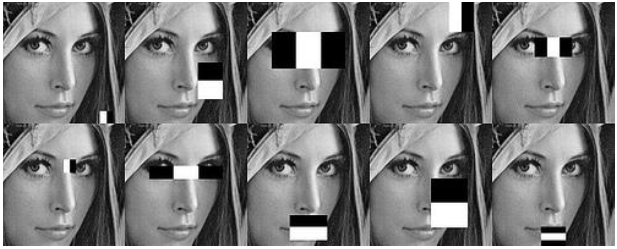
\includegraphics[width=90mm]{figures/Figure_chap2/haarf.PNG}
\caption{Features applied onto the face for matching facial characteristics}
\label{label_figure}
\end{figure}
The section \ref{subfig} shows how to put more than one pictures in one row.
\subsection{Subfigures}\label{subfig}
\begin{figure}[h]
\centering
\subfloat[Final 4 layers trainable.\label{cnf_mat_01}]{%
  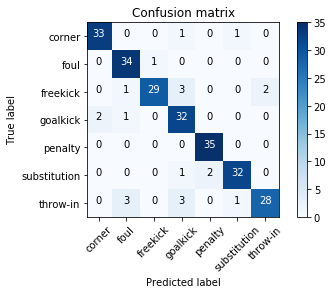
\includegraphics[width=0.5\textwidth]{figures/Figure_chap2/cnf_vgg16_4.png}%
}\hfil
\subfloat[Final 8 layers trainable.\label{cnf_mat_02}]{%
  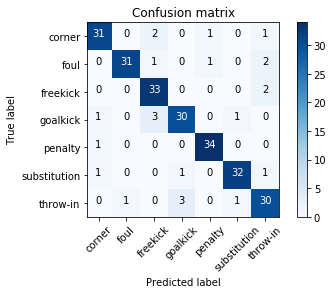
\includegraphics[width=0.5\textwidth]{figures/Figure_chap2/cnf_vgg16_8.png}%
}

\caption{VGG16 confusion matrix (a) final 4 layers trainable, (b) final 8 layers trainable.}
\label{fig_vgg16_cnf}
\end{figure}

\section{Table}
\subsection{soja table}
\section{Data collection of software modules}
\begin{table}[H]
\caption{Result of face, eye, and smile detection}
\label{swM1}
\begin{tabular}{|c|c|c|c|c|c|c|}
\hline
\multirow{2}{*}{\textbf{Participants}} & \multicolumn{2}{c|}{\textbf{Face Detection}} & \multicolumn{2}{c|}{\textbf{Eye Detection}} & \multicolumn{2}{c|}{\textbf{Smile Detection}} \\ \cline{2-7} 
                                       & \textbf{Total}      & \textbf{Detected}      & \textbf{Total}      & \textbf{Detected}     & \textbf{Total}       & \textbf{Detected}      \\ \hline
1                                      & 390                 & 385                    & 390                 & 375                   & 200                  & 180                    \\ \hline
2                                      & 425                 & 391                    & 425                 & 380                   & 223                  & 190                    \\ \hline
3                                      & 400                 & 375                    & 400                 & 370                   & 213                  & 183                    \\ \hline
4                                      & 401                 & 400                    & 401                 & 395                   & 200                  & 188                    \\ \hline
5                                      & 400                 & 380                    & 400                 & 377                   & 211                  & 187                    \\ \hline
6                                      & 430                 & 412                    & 430                 & 389                   & 209                  & 180                    \\ \hline
7                                      & 415                 & 400                    & 415                 & 379                   & 216                  & 170                    \\ \hline
8                                      & 401                 & 397                    & 401                 & 381                   & 219                  & 195                    \\ \hline
9                                      & 397                 & 393                    & 397                 & 379                   & 214                  & 187                    \\ \hline
10                                     & 396                 & 392                    & 396                 & 375                   & 207                  & 199                    \\ \hline
\textbf{mean}                          & 405.5               & 392.5                    & 405.5               & 380                   & 211.2                & 185.9                  \\ \hline
\textbf{variance}                      &                     & 114.9444444            &                     & 52                    &                      & 67.65555556            \\ \hline
\textbf{STDEV}                         &                     & 10.72121469            &                     & 7.211102551           &                      & 8.225299724            \\ \hline
\textbf{$\sqrt{N}$}                    & \multicolumn{6}{c|}{3.16227766}                                                                                                            \\ \hline
\textbf{$SEM$}           &                     & 3.390345771            &                     & 2.28035085            &                      & 2.601068157            \\ \hline
\end{tabular}
\end{table}
\subsection{kemon kemon table}

\begin{table}[H]
\centering
\caption{Quantitative data collection of three responsive behavior of the robot}
\label{aware1}
\rotatebox{90}{
\begin{tabular}{|c|c|c|c|c|c|c|c|c|c|c|}
\hline
\multirow{2}{*}{\textbf{\begin{tabular}[c]{@{}c@{}}\# of \\ Exp\end{tabular}}} & \multicolumn{5}{c|}{\textbf{Human Initiative Case}}                   & \multicolumn{5}{c|}{\textbf{Robot Initiative Case}}                  \\ \cline{2-11} 
                                                                               & \multicolumn{3}{c|}{\textbf{Methods}}   & \textbf{}    & \textbf{}    & \multicolumn{3}{c|}{\textbf{Methods}}   & \textbf{}    & \textbf{}    \\ \hline
\textbf{}                                                                      & \textbf{M1} & \textbf{M2} & \textbf{M3} & \textbf{Age} & \textbf{F/M} & \textbf{M1} & \textbf{M2} & \textbf{M3} & \textbf{Age} & \textbf{F/M} \\ \hline
1                                                                              & 1           & 1           & 1           & 22           & F            & 1           & 1           & 1           & 26           & F            \\ \hline
2                                                                              & 1           & 1           & 1           & 21           & F            & 1           & 1           & 1           & 24           & M            \\ \hline
3                                                                              & 1           & 1           & 1           & 21           & F            & 1           & 1           & 0           & 24           & F            \\ \hline
4                                                                              & 1           & 1           & 0           & 20           & F            & 1           & 1           & 0           & 27           & F            \\ \hline
5                                                                              & 1           & 1           & 0           & 22           & F            & 0           & 1           & 0           & 27           & M            \\ \hline
6                                                                              & 1           & 1           & 0           & 21           & F            & 0           & 1           & 0           & 27           & M            \\ \hline
7                                                                              & 1           & 1           & 0           & 21           & F            & 0           & 1           & 0           & 25           & F            \\ \hline
8                                                                              & 1           & 1           & 0           & 21           & F            & 0           & 0           & 0           & 22           & M            \\ \hline
9                                                                              & 1           & 1           & 0           & 21           & F            & 0           & 1           & 0           & 21           & F            \\ \hline
10                                                                             & 0           & 1           & 0           & 21           & F            & 1           & 1           & 1           & 21           & F            \\ \hline
11                                                                             & 0           & 1           & 0           & 21           & M            & 0           & 1           & 0           & 21           & F            \\ \hline
12                                                                             & 0           & 1           & 0           & 21           & M            & 1           & 1           & 1           & 20           & F            \\ \hline
13                                                                             & 0           & 1           & 0           & 21           & M            & 0           & 1           & 0           & 20           & M            \\ \hline
14                                                                             & 0           & 1           & 0           & 21           & M            & 1           & 0           & 0           & 20           & M            \\ \hline
15                                                                             & 0           & 1           & 0           & 21           & M            & 0           & 1           & 0           & 21           & M            \\ \hline
16                                                                             & 0           & 1           & 0           & 22           & M            & 0           & 1           & 0           & 21           & M            \\ \hline
Total                                                                          & 9           & 16          & 3           & 338          & M            & 7           & 14          & 4           & 367          &              \\ \hline
Mean                                                                           & 0.56        & 1           & 0.19        & 21.13        &              & 0.44        & 0.88        & 0.25        & 22.94        &              \\ \hline
STD                                                                            & 0.49        & 0           & 0.39        & 0.48         &              & 0.49        & 0.33        & 0.43        & 2.63         &              \\ \hline
\end{tabular}}
\end{table}
Table~\ref{aware1} example of normal table with multi row multi column with 90\degree rotation
\subsection{Sub table}\label{subtable}
\begin{table}[!htb]
    \caption{Global caption}
    \begin{subtable}{.5\linewidth}
      \centering
        \caption{}
        \begin{tabular}{ll}
            1 & 2
        \end{tabular}
    \end{subtable}%
    \begin{subtable}{.5\linewidth}
      \centering
        \caption{}
        \begin{tabular}{ll}
            3 & 4
        \end{tabular}
    \end{subtable} 
\end{table}

\chapter{Proposed Methodology/Framework/ Mechanism/ System Architecture}\label{chapter:chapter3}
\section{Algorithm \& Pseudo code \& Equations}
Package algorithm2e has been used here.
\subsection{Algorithm}
Canny edge detection is a popular multi-stage edge detection algorithm which was developed by John F. Canny in 1986 \cite{40}. 
\begin{algorithm}[ht]
\DontPrintSemicolon
\caption{Edge detection algorithm}
\SetAlgoLined
\KwInput{Gray Scale image}
\KwOutput{Image with thin line}
Calculate the gradient of all pixel in the X \& Y direction ($G_x$,$G_y$);

Compute magnitude and direction of each pixel( G, $\theta)$;\

Observe all nonmaximal value and reject them;\

Measure the high ($T_H$) and low($T_L$) thresholds using the histogram of the gradient magnitude of the image;\

\If{PixelValue>$T_H$}{
Consider the pixel as strong edge}
\ElseIf{($T_L$)< PixelValue <($T_H$)}
{Consider the pixel as weak edge}
\Else
{Reject}
\If{edge is strong edge}
{select the edge}
\ElseIf{Weak edge connected to any strong edge}
{select the edge}
\Else
{Reject}
\end{algorithm}
\subsection{Pseudo code}
\begin{algorithm}[ht]
\caption{Pseudocode}\label{euclid}
\begin{algorithmic}[1]
\Procedure{Psudocode}{}
\State $\textit{stringlen} \gets \text{length of }\textit{string}$
\State $i \gets \textit{patlen}$
\BState \emph{top}:
\If {$i > \textit{stringlen}$} \Return false
%\EndIf
\State $j \gets \textit{patlen}$
\BState \emph{loop}:
\If {$\textit{string}(i) = \textit{path}(j)$}
\State $j \gets j-1$.
\State $i \gets i-1$.
\State \textbf{goto} \emph{loop}.
\State \textbf{close};
%\EndIf
\State $i \gets i+\max(\textit{delta}_1(\textit{string}(i)),\textit{delta}_2(j))$.
\State \textbf{goto} \emph{top}.
\EndProcedure
\end{algorithmic}
\end{algorithm}
\subsection{Equations}
1st example:

\begin{algorithm}
\caption{Function}
  \begin{algorithmic}[1]
    \Function{Func\_name}{parameter}
      \State statement 1
      \State statement 2    
    \EndFunction
  \end{algorithmic}
\end{algorithm}

\begin{equation}
  h_{ij}= \dfrac{1}{2\pi\sigma^2} exp (-\dfrac{(i-(k+1))^2+(j-(k+1))^2}{2\sigma^2}; 1\le i, j\le (2k+1);
    \end{equation}
    2nd example:
    \begin{equation}
    \|Edge\_gradient(G)\|= \sqrt{I_x^2+I_y^2}
    Angle(\theta)= \tan^{-1}(\frac{I_y}{I_x})
\end{equation}
If you don't want to numbering any equation just use (\ no number) command.
\begin{equation}[H]
  SM1(x)=\begin{cases}
    Stops, & \text{if $\alpha=1$}.\\
    Moves, & \text{otherwise}.
  \end{cases}
  \nonumber
\end{equation}
\begin{equation}
  SM2(x)=\begin{cases}
  \mbox{\textit{Nod thrice}}, & \text{if $\beta=1$}.\\
   \mbox{\textit{Nods once}}, & \text{if $\beta=2$}\\
    \mbox{\textit{No movement}}, & \text{otherwise}.
  \end{cases}
  \nonumber
\end{equation}
\subsection{Matrix}[H]
 $$
 K_x=\begin{bmatrix} 
-1 & 0 & 1 \\
-2 & 0 & 2\\
-1 & 0 & 1
\end{bmatrix}
 K_y=\begin{bmatrix}
1 & 2 & 1 \\
0 & 0 & 0\\
-1 & -2 & -1
\end{bmatrix}
$$
\section{Flow chart}
\subsection{arrow and square}
\tikzstyle{ellip}=[draw,ellipse,fill=white!20,minimum height=2em]
\tikzstyle{rec}=[draw,rectangle,fill=white!20,text width=6em,text centered,minimum height=2em]
\tikzstyle{line}=[draw,-latex']
\begin{figure}[htbp]
\begin{center}
\begin{tikzpicture}[]

\node[ellip](step1) at (2,0){Start};
\node[rec] (step2) at (-1,-1) {Launch Speech to Text};
\node[rec] (step3) at (5,-1) {Launch Sign Language Keyboard};
\node[rec] (step4) at (-1,-3.3) {Speech to Sign Language Conversion with Help of Virtual Agent};
\node[rec] (step5) at (5,-3.5) {Convert Bangla Text};
\node[ellip] (step6) at (2,-4.7) {End};

\path[line] (step1) -| (step2);
\path[line] (step1) -| (step3);
\path[line] (step2) -- (step4);
\path[line] (step3) -- (step5);
\path[line] (step4) |- (step6);
\path[line] (step5) |- (step6);

\end{tikzpicture}
\end{center}
\caption{Overview of the proposed system}
\label{fig:first}
\end{figure}
\subsection{another example}
\tikzstyle{ellip}=[draw,ellipse,fill=white!20,minimum height=1em,minimum width=7.1em]
\tikzstyle{rec}=[draw,rectangle,fill=white!20,text width=6em,text centered,minimum height=2em]
\tikzstyle{line}=[draw,-latex']
\tikzstyle{line2}=[draw]
\tikzstyle{rec2}=[draw=white,rectangle,fill=white!20,text width=6em,text centered,minimum height=2em]
\begin{figure}[htbp]
\begin{center}
\begin{tikzpicture}[]

\node[rec] (step1) at (-1,0) {Speaking Bangla};
\node[rec] (step2) at (2,0) {Splitting Words from Sentence};
\node[rec] (step3) at (5,0) {Splitting suffixes};
\node[rec] (step4) at (5,-2) {Fetching Sign};
\node[rec] (step5) at (-1,-2) {Sign Language Output};
\node[rec2] (step7) at (2,-2){Raw folder containing animation};
\node[ellip] (step6) at (2,-1) {};

\path[line] (step1) -- (step2);
\path[line] (step2) -- (step3);
\path[line] (step3) -- (step4);
\path[line2] (step4) -- (5,-3);
\path[line] (5,-3) -| (step5);
\path[line2] (3.05,-1) -- (3.05,-2.8);
\path[line2] (3.05,-2.8) -- (0.95,-2.8);
\path[line2] (0.95,-2.8) -- (0.95,-1);
\draw[>= open triangle 45, <->](step4) -- (3.05,-2);
\end{tikzpicture}
\end{center}
\caption{Layout for showing the signs on the mobile screen}
\label{fig:second}
\end{figure}

\chapter{Implementation }\label{chapter:chapter4}
\input{chapters/Chapter4}

\chapter{Experimental Result analysis and Evaluation}\label{chapter:chapter5r}
\input{chapters/Chapter5}

\chapter{Conclusion}\label{chapter:chapter6} 
\input{chapters/Chapter6}

\pagebreak
\phantomsection
\addcontentsline{toc}{chapter}{Bibliography}
\nocite{*}
\printbibliography
\pagebreak
\phantomsection

%\addcontentsline{toc}{chapter}{Appendix}\label{chapter:appendix-one}
\begin{appendices}
\titleformat{\chapter}[display]
{\bfseries\Large} %
{\begin{tabularx}{\linewidth}{@{}Xl@{}}
\raisebox{3ex}{\rule[-1.8ex]{\linewidth}{5pt}}%\vspace{1.5ex}%
 & \textsuperscript{\fontsize{30}{60}\selectfont{Appendix}}%
{\fontsize{70}{60}\selectfont\thechapter}\end{tabularx}} %
{10 pt}%
{\bfseries\fontsize{25}{20}\selectfont}%
%\setcounter{Appendix}{0}

\chapter{} 
\renewcommand{\thesection}{A.\arabic{section}}
%\chapter{}
%\chapter{Appendix}
This Appendix presents the overall data analysis of the three software modules. In first section face, eye and smile detection result is analyzed and in the second section gaze tracking module has been discussed. 
\section{first appendix data}\label{appendixA1}

\section{Second data collection}\label{appendixA2}

\chapter{}
\renewcommand{\thesection}{B.\arabic{section}}
%{\let\clearpage\relax\chapter*{Appendix B}}

Another appendix section
\section{Another data}\label{appendixB1}

% Please add the following required packages to your document preamble:
% \usepackage{booktabs}


\section{Another data  2}\label{appendixB2}
 
\chapter{}
%{\let\clearpage\relax\chapter*{Appendix C}}
\renewcommand{\thesection}{C.\arabic{section}}
This appendix includes the data of final results.
\section{Final data appendicx}\label{appendixC}

\end{appendices}
\end{document}